\documentclass[a4paper, 11pt]{article}
\usepackage{fontspec}
\usepackage{polyglossia}
\usepackage{graphicx}
\setmainlanguage{mongolian}
\setmainfont{Noto Sans} 
\setsansfont{Arial}     
\setmonofont{Courier New} 

\begin{document}

\begin{center}
    {\large \textbf{ШИНЖЛЭХ УХААН ТЕХНОЛОГИЙН ИХ СУРГУУЛЬ}}\\[0.3cm]
    {\large Мэдээлэл холбооны технологийн сургууль}\\[1.2em]
\vspace{1cm}
    
\includegraphics[width=1.08in, height=2.05in]{MustLogo.png}\\[1.2em]
\vspace{2cm}
    {\Huge \textbf{GYM MEMBERSHIP SYSTEM ТӨСЛИЙН ТАЙЛАН}}
\end{center}

\vspace{3cm}
\begin{flushleft}
\vspace*{\fill} 
\hspace*{0pt}Хичээл заасан багш: А.Отгонбаяр \\
\hspace*{0pt}Оюутан: Г.Анужин B242270051 \\
\hspace*{0pt}Оюутан: А.Аминхишиг B242270011 \\
\hspace*{0pt}Оюутан Ж.Мэнд-Амгалан B242270008\\
\end{flushleft}
\vspace{2cm}
\item 

\section*{Төслийн танилцуулга}
Gym Membership төсөл нь фитнесийн гишүүнчлэлийн мэдээллийг удирдах програм юм. Энэхүү систем нь гишүүдийн бүртгэл, гишүүнчлэлийн хугацаа зэрэг үндсэн үйлчилгээг автомажуулсан.
\subsection*{Гол онцлогууд нь:}
\begin{itemize}
\item Гишүүдийн бүртгэл, шинэчлэлт
\item Гишүүнчлэлийн хугацааны автомат тооцоолол 
\item Тайлан гаргах боломж
\end{itemize} 
\subsection*{Шаардлагын тодорхойлолт}
\begin{itemize}
\item Гишүүнчлэлийн мэдээлэл хадгалах (нэр, дугаар, төрөл, и-мэйл)
\item Гишүүнчлэлийн төрөл (энгийн/VIP)
\item Гишүүнчлэлийн дуусах хугацаа автомат тооцоолох
\item Гишүүдийн мэдээлэл шинэчлэх/устгах
\item Алдагдсан карт дахин олгох 
\end{itemize}
\subsection*{Кодын дизайн, бүтэц}
Систем нь дараах 2 гол класс-уудаас бүрдэнэ:

\begin{figure}[h!]
    \centering
    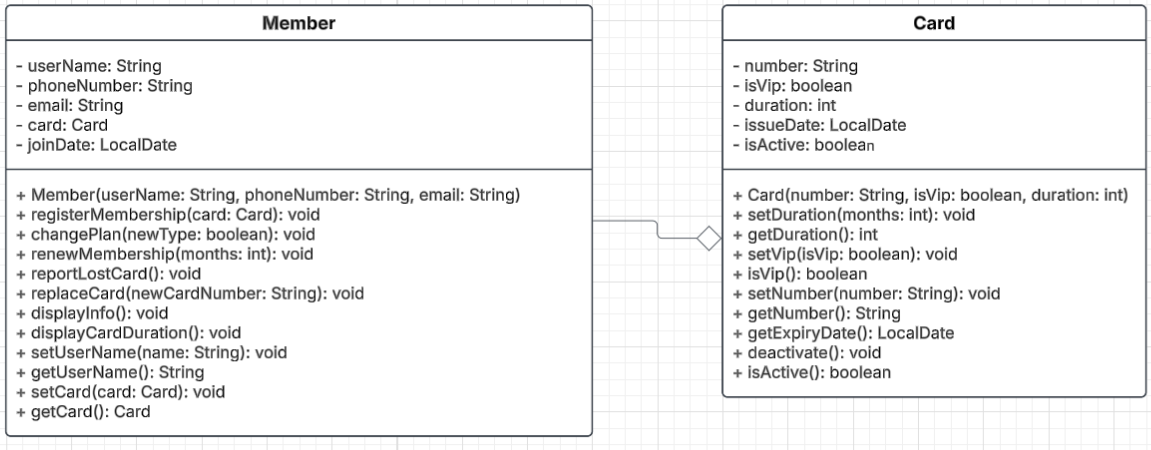
\includegraphics[width=1\linewidth]{umldiagram.png}
    \caption{Системийн UML диаграм}
    
\end{figure}

\subsection*{Сурсан мэдсэн зүйл: }
\begin{itemize}
\item Төслийн загвар, шинжилгээ боловсруулах
\item TDD ( Test-Driven Development) аргачлалд суралцсан
\end{itemize}
\subsection*{Бэрхшээлтэй зүйлс: }
\begin{itemize}
\item Алдагдасан карт дахин олгох шаардлагатай байсан
\item Гишүүнчлэлийн хугацааг тооцоход LocalDate болон Date ялгаа
\end{itemize}
\subsection*{Цаашдын хөгжүүлэлт: }
\begin{itemize}
\item График интерфэйс нэмэх
\item Гишүүнчлэлийн хугацаа дуусах үед цахим шуудангаар мэдэгддэг болгох
\end{itemize}
\subsection*{Card class methods}

\begin{description}
    \item {public Card (String number, boolean isVip, int duration)}
\item  -Шинэ гишүүнчлэлийн карт үүсгэх
    \begin{itemize}
        \item number: Картын дугаар
        \item isVip: VIP эсэх төлөв
        \item duration: Гишүүнчлэлийн хугацаа
    \end{itemize}
    
    \textbf{Алдаа:} Хэрэв дугаар хоосон эсвэл хугацаа 0-ээс бага бол IllegalArgumentException. 
    
    \textbf{Лог:} Шинэ карт үүссэн тухай мэдээлэл
    
    \item {public void extendDuration(int months)}
    \item -Гишүүнчлэлийн хугацааг сунгах
    \begin{itemize}
    \item  months - нэмэх сарын тоо
     \end{itemize}
    \textbf{Алдаа:} Хэрэв сарын тоо 0-ээс бага бол алдаа
    
    \textbf{Лог:} Хугацаа сунгагдсан тухай мэдээлэл
    
    \item {public void deactivate()}
    - Картыг идэвхгүй болгох
    
    \textbf{Лог:} Карт идэвхгүй болсон тухай мэдээлэл
\end{description}
\subsection*{Member class methods}
\begin{description}
    \item{public Member(String name, String phone, String email)}
    \item -Шинэ гишүүн бүртгэх

    \begin{itemize}
        \item name: Гишүүний бүтэн нэр
        \item phone: Утасны дугаар
        \item email: И-мэйл хаяг
    \end{itemize}
    
    \textbf{Алдаа:} Хэрэв ямар нэг талбар хоосон бол IllegalArgumentException шидэнэ
    
    \textbf{Лог:} Шинэ гишүүн бүртгэгдсэн тухай мэдээлэл
    
    \item {public void registerMembership(Card card)}
    Гишүүнд карт оноох
    \begin{itemize}
    \item card - гишүүнчлэлийн карт
     \end{itemize}
    \textbf{Алдаа:} Хэрэв карт null бол алдаа шидэнэ
    
    \textbf{Лог:} Гишүүнд карт оноогдсон тухай мэдээлэл
    
    \item{public void renewMembership(int months)}
    \item -Гишүүнчлэлийн хугацааг сунгах
     \begin{itemize}
    \item months - нэмэх сарын тоо
     \end{itemize}
    \textbf{Алдаа:}
    \begin{itemize}
        \item Хэрэв карт бүртгэгдээгүй бол IllegalStateException
        \item Хэрэв сарын тоо 0-ээс бага бол IllegalArgumentException
    \end{itemize}
    
    \textbf{Лог:} Гишүүнчлэл сунгагдсан тухай мэдээлэл
    
    \item{public void reportLostCard()}
    Картыг алдсан мэдээлэх
    
    \textbf{Алдаа:} Хэрэв карт бүртгэгдээгүй бол IllegalStateException
    
    \textbf{Лог:} Карт алдагдсан тухай warning мэдээлэл
\end{description}
\subsection*{Log4j2 Ашиглалт}
Системд org.apache.logging.log4j санг ашигласан:

\begin{itemize}
    \item \texttt{logger.info()}: Ердийн үйлдлийн мэдээлэл
    \item \texttt{logger.warn()}: Анхааруулга мэдээлэл
    \item \texttt{logger.error()}: Алдааны мэдээлэл
\end{itemize}

\subsection*{Лог Формат}
Лог бүрт дараах мэдээлэл автоматаар бүртгэгдэнэ:

\begin{itemize}
    \item Хугацаа
    \item Логийн түвшин (INFO, WARN, ERROR)
    \item Классын нэр
    \item Үйлдлийн дэлгэрэнгүй мэдээлэл
\end{itemize}

\subsection*{Алдааны Удирдлага}
Системд дараах төрлийн алдаануудыг зохицуулсан:

\begin{itemize}
    \item {IllegalArgumentException}: Буруу параметр оруулсан
    \item {IllegalStateException}: Буруу төлөвт байгаа үед
    \item {NullPointerException}: Null утга дамжуулсан
\end{itemize}

Алдаа бүрт холбогдох лог бүртгэгдэж, хэрэглэгчид ойлгомжтой алдааны мессеж илгээгдэнэ.

\end{document}